%------------------------------------------------------------
%------------------------------------------------------------
\section{University Timetabling Problem}
\label{sec:schema}
A \UTP{} instance is defined by an entity model and a rules set. %and a solution. % and a pre-assignment. 
%The entity model defines the schedule horizon, courses and resources of the instance and encodes core constraints relating to session scheduling, resource allocation, and student sectioning.
%Rules express additional constraints meant to capture stakeholder requirements on particular aspects of the problem.
%A rule is a conjunction of constraints built from a catalog of timetabling-specific predicates.
%The solution is a list of choices made for some or all of the decisions at stake (e.g., start time of a session).
%Note that a \UTP{} instance may have no rules.% rules set and solution components may be omitted. 
% Besides, the listed solution is not required to be consistent with the constraints enforced by the entity model or the rules set.
% This allows to tackle subproblems using separate instances and to support timetable generation or repair tasks.
% Each rule is an intensional representation of a collection of constraints applying to different entities.
% {\UTP} instances may thus be compiled to lower-level representations that explicitly declare all constraints and whose format is compatible with {\CP} languages.
%{\UTP} instances may therefore be compiled into lower-level representations that lists all constraints and whose format is tailored to back-end solvers.
%
A solution to a \UTP{} instance is a list of choices made for all the decisions at stake %(e.g., start time of a session).
that satisfies the core constraints of the entity model and the constraints expressed by the rules.
%Note that a \UTP{} instance may have no rules and an input solution may be provided based on context.
%We defined \acronym{XUTP}, an embedded version of the \UTP{} language into \XML{}.
%We do not provide here the detailed \XML{} specification of \acronym{XUTP} (see~\cite{uspSite}).
We provide in this section an informal description and set-theoretic semantics for the \UTP{} language components, namely the entity model (Section~\ref{sec:entity-model}), constraints (Section~\ref{sec:constraints}), rules (Section~\ref{sec:rules}) and solution (Section~\ref{sec:solution}).
Section~\ref{sec:related-work} draws a comparison between the \UTP{} language and the \ITC{} schema.


%
%We present theses components in turn, 
%discuss the type of features and requirements that may be factored in,
%and provide set-theoretic semantics for the rules language and flattening process.
%The reader is referred to \cite{uspSite} for the detailed {\XML} specification of {\XUTP} and the {\JSON/\DZN} instance formats.
%\cite{uspSite} also provides access to the {\MINIZINC} and {\CHR} models, the tool suite, and a benchmark of instances.
%motivate design choices,
%whose {\CP} implementation is addressed in Section~\ref{sec:model}.

%motivate design choices, 
%and highlight differences with related work.

%------------------------------------------------------------
%------------------------------------------------------------
\subsection{Entity model}
\label{sec:entity-model}
The entity model of a {\UTP} instance defines its schedule horizon, course structure and resources, as well as properties of entities and relational maps (see 
Figure~\ref{fig:utp-entity-model} for a sketch of the meta-model and Figure~\ref{fig:utp-rule-1} for a toy example).  
First, the entity model uses a time grid that decomposes into weeks, weekdays and daily slots. %, the number of which is instance-specific. 
Weeks share the same weekdays and weekdays the same daily slots. The latter make up 24 hours and have the same duration. %measured in minutes. 
Note that neither successive weeks nor successive weekdays are assumed to be consecutive. %and that Monday is the first weekday by convention. 
The schedule horizon is implicitly defined by the series of time slots mapping to week, weekday and daily slot combinations. Slots hence serve as time points to represent start and end times of course sessions and to measure session duration, travel time and any gap between sessions.

% % For one-column wide figures use
% \begin{figure}[h]
% % \includegraphics{utp-time-grid.eps}
% \caption{{\UTP} 3-layered time grid}
% \label{fig:utp-time-grid}
% \end{figure}

Courses have a tree-structure wherein each course (e.g., Algorithms) decomposes into parts (e.g., Lecture and Lab), parts into classes (e.g., lecture classes A and B), and classes into sessions (e.g., sessions 1 to 10 for each lecture class). Class sessions are the elementary tasks to schedule when solving a {\UTP} instance and the model fixes their number, duration and sequencing. First, the classes of a course part are decomposed into an identical number of sessions of equal duration, both constants being part-specific. Although this approach forbids classes using different session durations in a course part, 
%it %provides flexibility for handling sessions independently wrt. scheduling and resource allocation.
%Fixed decompositions also 
it is paramount to capture requirements that rely on clear-cut sessions (e.g., starting lab classes after 2 lecture sessions, synchronizing the 5th sessions of the lab classes for a joint examination). Second, the sessions of a class are ranked in the model and must be sequenced accordingly in any solution (session 1 before session 2 \ldots). Note that sessions are considered uninterruptible and, in particular, may not overlap two days. 

\begin{figure}[ht]
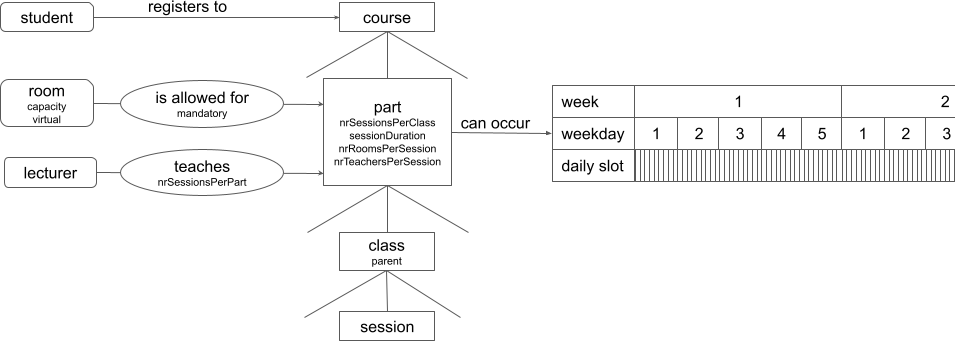
\includegraphics[scale=0.35]{img/utp_entity_model.png}
\caption{Entity meta-model.}
\label{fig:utp-entity-model}
\end{figure}

{\UTP} resources fall into 4 types, namely, rooms, lecturers, students and (student) groups.
All the resources of an instance, except groups (see Section~\ref{sec:solution}), are declared and typed in the entity model. In practice, upstream processes and decisions %constrain the resourcing and timing of courses.
%Basic restrictions come in the form of compatibility constraints that list 
determine the suitable rooms, eligible lecturers, candidate students and allowed times for the different courses (e.g., faculties prescribing degree-specific time grids, departments implementing room pooling policies and naming lecturers for courses, students registering to courses). %Such constraints are built in the entity model but scoped differently depending on resource types. %Specifically, 
These compatibility constraints are modeled by associating sets of possible start times, rooms and lecturers to each course part and a set of registered students to each course. Each session then inherits the sets of allowed resources from the course part and the course it belongs to.
%and which are implicitly the sessions.
%Student registrations are listed separately and %the possible students for a session are those registered to the course it sits in.
%any student registered to a course is considered a possible candidate for each of its sessions.

The entity model also encodes flow constraints that govern the distribution of resources over courses based on student registrations and capacity planning decisions (e.g., workload distribution between lecturers). First, each lecturer is allocated a fixed number of sessions in each course part he is eligible for, leaving lecturer-to-session assignment decisions to solvers. Second, each room allowed in a course part may be freely allocated to any session of the part (possibly none) but the model provides the flexibility to mark a room as mandatory in which case it will host or co-host all the sessions. As for students, the sectioning policy is implicit and complies with the course structure, i.e., each student must be assigned to a single class in each part of a course he has registered to and attend all sessions of these classes. In addition, the model supports group nesting constraints between classes to implement course-specific policies (e.g., aggregating student groups bottom-up from labs to lectures) or cross-course sectioning (e.g., imposing the same groups between classes of different courses of a curriculum).
 
Resource utilization is naturally subject to demand and capacity constraints.
Since modalities differ from one environment to the next, the language supports disjunctive and cumulative resources. The default policy is to consider all students, groups, lecturers and rooms as cumulative resources, i.e., they can attend, teach or host simultaneous sessions. Note though that rules may be stated to make some resources fully disjunctive or to prevent specific sessions from overlapping. Support for cumulative resources is paramount to address flexible attendance requirements (e.g., students assigned optional tutoring sessions that may overlap with compulsory courses) or to handle multi-class events (e.g., rooms hosting several classes for an exam or a conference). The model imposes no limits on the number of parallel sessions lecturers and students may attend. Rooms however may only host class sessions whose cumulated headcount is within their capacity. Upper bounds on room capacity and class size are encoded for all rooms and classes and the model also allows uncapacitated rooms to cater for the case of virtual rooms.

The language also supports sessions using multiple resources of the same type. %at any point in time.
The need for multiple rooms or lecturers arises in practical situations (e.g., multi-room sessions for hybrid teaching, joint supervision of practical work sessions, exams requiring several monitors). %and the number of resources required per session is course part dependent.
%such restrictions are expressed in the entity model through cardinality constraints. %that are lifted to course parts. 
To this end, the model associates to each course part the number of lecturers required per session 
and indicates whether the sessions are single- or multi-rooms.
Note that sessions without lecturers or rooms are allowed (e.g., unsupervised student project sessions).
The model enforces specific constraints to handle multi-room sessions which override the default room allocation policy. Specifically, students attending the session may be freely dispatched in rooms irrespectively of the group structure, the cumulated capacity of the allocated rooms is taken into account for hosting, uncapacitated rooms cannot be allocated, and 
the allocated rooms are considered disjunctive for the time of the session.
%a {\UTP} instance may freely mix single- and multi-resource sessions as well as disjunctive and cumulative resources. 

Note finally that the language provides users with the ability to label resources and course elements to define their own classes of entities (e.g., teams of lecturers, blocks of rooms). Labels together with built-in entity types and identifiers are used to filter entities and to scope rules appropriately.
 


We formalize below the entity model and introduce notations that will be used thereafter.
Let ${\ENTITY}$ denote the set of entities
and ${\SESSION}$ the set of sessions.
${\ENTITY}$ is partitioned into   
a set of courses ${\COURSE}$, 
a set of course parts ${\PART}$, 
a set of classes ${\CLASS}$, 
a set of students ${\STUDENT}$, 
a set of lecturers ${\TEACHER}$,
a set of rooms ${\ROOM}$,
and the singleton domain of courses ${\COURSES}$ 
(${\COURSES}=\myset{\COURSE}$). 
Let 
%${\COURSES}$ denote the course domain, 
%${\COURSE}$ the set of courses (${\COURSES}=\myset{\COURSE}$), 
%${\PART}$ the set of course parts, 
%${\CLASS}$ the set of classes, 
%${\SESSION}$ the set of sessions, 
%${\STUDENT}$ the set of students, 
%${\TEACHER}$ the set of teachers, 
%and 
%${\ROOM}$ the set of rooms.
$
{\TYPE}
=
\myset{
{\COURSES}, 
{\COURSE},
{\PART},
{\CLASS},
{\STUDENT},
{\TEACHER},
{\ROOM}
}
$
denote the set of entity types
(${\ENTITY}=\setunion{X}{\TYPE}{X}$)
and 
$
{\prec}
=
\myset{
({\COURSES},{\COURSE}),
({\COURSE},{\PART}),
({\PART},{\CLASS}),
({\CLASS},{\SESSION}),
({\STUDENT},{\COURSE}),
$
$
({\TEACHER},{\PART}),
({\ROOM},{\PART})
}
$
denote the relation over 
${\TYPE}\cup\myset{\SESSION}$ 
that models the course hierarchy
and the distribution of resource types over course components.

${\prec^{*}}$
%${\preceq^{*}}$
denotes the transitive %and reflexive 
closure of
${\prec}$ 
over
${\TYPE}\cup\myset{\SESSION}$
and
${\maptype{X}{Y}}:X\rightarrow2^{Y}$
denotes the function mapping each element of $X$ to its set of compatible elements in $Y$
for each pair %$(X,Y)$ such that 
%$X{\preceq^{*}}Y$.
$X{\prec^{*}}Y$.
For instance, 
${\maptype{\ROOM}{\PART}}$ 
represents the distribution of rooms over course parts, 
${\maptype{\PART}{\CLASS}}$ 
the decomposition of course parts into classes,
${\maptype{\CLASS}{\SESSION}}$ 
the decomposition of classes into sessions,
and ${\maptype{\ROOM}{\SESSION}}$ 
the inferred distribution of rooms over sessions.
The functions corresponding to the pairs of $\prec$
are directly encoded in the entity model
and the remaining functions are defined inductively using recursive aggregation. 

We shall denote by ${\map{X}{Y}{i}}$ the image of entity $i$ of type $X$ over $2^Y$ %, i.e., the set of elements of type $Y$ compatible with $i$. 
and by ${\maptype{Y}{X}}$ the inverse of ${\maptype{X}{Y}}$.
Equation (\ref{model:hierarchy}) below models the hierarchical decomposition of course elements\footnote{$\sqcup$ denotes the disjoint union operation, i.e. set union over pairwise disjoint sets.},
Equation (\ref{model:transitivity}) is the closure rule over 
%$\preceq^{*}$. 
$\prec^{*}$,
%Note that each map $\maptype{\SESSION}{X}$ is the inverse of map $\maptype{X}{\SESSION}$.
and Equation (\ref{model:inverse}) models inverse maps.

\begin{align}
%
\forall (X,Y) \in 
\myset{
({\COURSES},{\COURSE}),
({\COURSE},{\PART}),
({\PART},{\CLASS}),
({\CLASS},{\SESSION})
}:
Y=
\setpartition{i}{X}{\map{X}{Y}{i}} 
\label{model:hierarchy}
\\
%
\forall X,Y,Z \in {\TYPE}\cup\myset{\SESSION}:
X\preceq^{*} Y\preceq^{*} Z 
\Rightarrow 
(\forall i \in X:
\map{X}{Z}{i}=\setpartition{j}{\map{X}{Y}{i}}{\map{Y}{Z}{j}}
\label{model:transitivity})
\\
%
\forall X,Y \in {\TYPE}:
X\preceq^{*} Y 
\Rightarrow 
(\forall i \in X, j \in Y:
j \in \map{X}{Y}{i} \Leftrightarrow i \in \map{Y}{X}{j}
)
\label{model:inverse}
%\\
%%
%\forall X \in {\TYPE}\cup\myset{\SESSION},
%i \in X:
%\domarg{X}{X}{i} = \myset{i} \label{model:selfmap}
%%
\end{align}



\begin{table}[ht]
\begin{center}
\begin{tabular}{|rl|}
\hline
$(\WEEK,\WEEKDAY,\DAILYSLOT)$               & the number of weeks $\WEEK$, weekdays $\WEEKDAY$ and daily slots $\DAILYSLOT$
\\
$\SLOT$                                     & the time slots 
\\\hline
$\ENTITY$                                   & the entities
\\
$\COURSES\subseteq\ENTITY$                  & the course domain
\\
$\COURSE\subseteq\ENTITY$                   & the courses
\\
$\PART\subseteq\ENTITY$                     & the course parts
\\
$\CLASS\subseteq\ENTITY$                    & the classes
\\
$\ROOM\subseteq\ENTITY$                     & the rooms
\\
$\TEACHER\subseteq\ENTITY$                  & the lecturers
\\
$\STUDENT\subseteq\ENTITY$                  & the students
\\
$\map{X}{Y}{i}\subseteq{Y}$                 & the entities of type $Y$ associated with entity $i$ of type $X$
\\\hline
${\LABEL}\subseteq2^{{\ENTITY}}$            & the labels
\\\hline
$\GROUP\subseteq{2^{\STUDENT}}$             & the groups of students
\\\hline
$\SESSION$                                  & the sessions
\\
$\map{X}{\SESSION}{i}\subseteq{\SESSION}$   & the sessions compatible with entity $i$ of type $X$
\\
$\map{\SESSION}{X}{s}\subseteq{X}$          & the entities of type $X$ compatible with session $s$
%\\
%$\disjunctiverooms\subseteq{\ROOM}$         & the set of disjunctive rooms
\\
$\partallowedslots{s}\subseteq{\SLOT}$      & the start times allowed for session $s$
\\
$\sessionduration{s}\in{\SLOT}$             & the duration of session $s$
\\
$\sessionrank{s}\in{\NATURAL^*}$            & the rank of session $s$ in its class
\\
$\sessionranked\subseteq{\SESSION\times\SESSION}$ & the pairs of sessions with consecutive ranks in a class
\\\hline
$\classparents{k}\subseteq{\CLASS}$          & the parent classes of class $k$ if any
\\
$\classcapacity{k}\in{\NATURAL}$            & the maximum size of class $k$
\\\hline
$\roomcapacity{r}\in{\NATURAL}$             & the capacity of room $r$
\\
$\virtualroom{r}\in{\BOOLEAN}$              & whether room $r$ is virtual or not
\\
$\virtualrooms\subseteq{\ROOM}$             & the virtual rooms
\\\hline
$\multiroompart{p}\in{\BOOLEAN}$            & whether course part $p$ is multi-room or not
\\
$\multiroomparts\subseteq{\PART}$           & the multi-room parts
\\
$\mandatoryrooms{p}\subseteq{\ROOM}$        & the mandatory rooms of part $p$
\\
$\partteachermultiplicity{p}\in{\NATURAL}$  & the number of lecturers required by every session of part $p$
\\
$\partteacherservice{l,p}\in{\NATURAL}$     & the number of sessions required by lecturer $l$ in part $p$
\\
\hline
\end{tabular}
\caption{Entity model: constants, sets, maps and relations.}
\label{table:model-maps}
\end{center}
\end{table}


Table~\ref{table:model-maps} provides the full list of constants, sets, properties and relational maps encoded in the entity model.\footnote{
The following rules apply. $\SLOT=\myset{i.\WEEKDAY.\DAILYSLOT+j.\DAILYSLOT+k\ |\ 0\leq i<\WEEK,0\leq j<\WEEKDAY,1\leq k\leq\DAILYSLOT}$.
For each class $k$ in part $p$,
$\myset{\sessionrank{s}\ |\ s\in\map{\CLASS}{\SESSION}{k}}=\myset{1,\ldots,\mycard{\map{\CLASS}{\SESSION}{k}}}$, 
%$\mycard{\classparents{k}}\leq1$ 
and $\classparents{k}\not\subset\map{\PART}{\CLASS}{p}$.
For each pair of sessions $s,s'$, 
$(s,s')\in\sessionranked$ iff $\map{\SESSION}{\CLASS}{s}=\map{\SESSION}{\CLASS}{s'}$ and $\sessionrank{s'}=\sessionrank{s}+1$.
For each course part $p$,
%$p\in\multiroomparts$ iff $\multiroompart{p}$; 
%and 
$\partteachermultiplicity{p}.\mycard{\map{\PART}{\SESSION}{p}}=\sum\limits_{l\in\map{\PART}{\TEACHER}{p}}{\partteacherservice{l,p}}$.}

%We shall denote by
%${\RANK}$
%the range of session ranks,
%${\maptype{\RANK}{\SESSION}}:\RANK\rightarrow2{^\SESSION}$
%the rank-based partitioning of sessions,
%and
%${\LABEL}$
%the set of labels 
%(${\LABEL}\subseteq2^{{\ENTITY}}$)
%completed 
%with the whole set of entities %to mock label optionality
%($\ENTITY\in{\LABEL}$)
%and singleton entities %to support identity-based selection
%($\myset{\myset{e}\ |\ e\in{\ENTITY}}\subseteq{\LABEL}$).
%As discussed in section~\ref{sec:rules},
%labels are optional filters used in rules to select entities
%hence the formal inclusion of $\ENTITY$ in ${\LABEL}$ to mock label optionality.
%Likewise, entity identifiers are used as an alternative to labels
%hence the inclusion of singleton entities in ${\LABEL}$.

%------------------------------------------------------------
%------------------------------------------------------------
\subsection{Predicates and constraints}
\label{sec:constraints}
{\UTP} constraints apply to pairs, called e-maps, which associate an entity with a non-empty subset of its compatible sessions.
%which we call e-maps. 
Constraints are built with predicates whose signature includes e-map variables%ranging over the set of e-maps
, the number of which is referred to as the arity of the predicate. 
Note that some predicates may also accept parameters.
Let 
${\EMAP}=
\setunion{X}{\TYPE}
\myset{(e,S')\ |\ e\in X,S'\subseteq\map{X}{\SESSION}{e}\wedge S'\neq\emptyset}$
denote the set of e-maps,
a {\UTP} constraint has the form
\begin{align}
c((e_1,S_1),\ldots,(e_m,S_m),p_1,\ldots,p_n) \label{rule:constraint}
\end{align}
where 
$c$ is a predicate symbol of arity $m$,
$(e_1,S_1),\ldots,(e_m,S_m)$ are e-maps ($(e_i,S_i)\in{\EMAP}$, $i=1\ldots m$) 
and 
$p_1,\ldots,p_n$ are values for the parameters of $c$ ($n\geq0$).
Three constraints (\ref{constraint-example-1}, \ref{constraint-example-2}, \ref{constraint-example-3}) are illustrated in Figure~\ref{fig:utp-rule-1}.


Every predicate may be used indistinctly with e-maps defined on course elements or on resources.
E-maps defined on resources are interpreted as conditional session-to-resource assignments
when checking constraints 
whereas e-maps defined on course elements are unconditional assignments since they model constitutive sessions.
In other words, 
a constraint is only evaluated
on the sessions for which its e-map arguments and the considered solution propose the same entity assignment.\footnote{Formally, let $\var{E}{\SESSION}{e}$ be the variable denoting the set of sessions assigned to entity $e$ and $S'_1,\ldots,S'_m$ be sets of sessions, the conditionality of a constraint $c$ is stated as follows: 
$(\var{E}{\SESSION}{e_1}=S'_1 \wedge\ldots\wedge\var{E}{\SESSION}{e_m}=S'_m)
\Rightarrow
(c((e_1,S_1),\ldots,(e_m,S_m),p_1,\ldots,p_n)
\Leftrightarrow
c((e_1,S_1\cap S'_1),\ldots,(e_m,S_m\cap S'_m),p_1,\ldots,p_n))$.}

It follows that 
a constraint is evaluated on every session that is mapped to a course element by one of its e-map arguments.
Constraints that apply exclusively to course elements are therefore unconditional. 
Note also that the use of e-maps that model the whole set of sessions compatible with an entity 
will necessarily constrain any session that may be assigned to this entity.


%Every predicate may be used indistinctly with e-maps defined on course elements or on resources which we call c-maps and r-maps, respectively. R-maps are interpreted conditionally since they map a resource to some of its possible sessions whereas c-maps model unconditional assignments since they model constitutive sessions of course elements. In other words, a constraint must be evaluated on every session of every c-map in its scope but only on the sessions of its r-maps whose resource assignment is compatible with the proposed solution.\footnote{Formally, let $\var{E}{\SESSION}{e}$ be the variable denoting the set of sessions assigned to entity $e$ and $S'_1,\ldots,S'_m$ be sets of sessions, the conditionality of a constraint $c$ is stated as follows:  $(\var{E}{\SESSION}{e_1}=S'_1 \wedge \var{E}{\SESSION}{e_m}=S'_m) \Rightarrow (c((e_1,S_1),\ldots,(e_m,S_m),p_1,\ldots,p_n) \Leftrightarrow c((e_1,S_1\cap S'_1),\ldots,(e_m,S_m\cap S'_m),p_1,\ldots,p_n))$.}
%effectively assigns to the resource of the r-map.
%(see Rule (\ref{rule:conditionality})).
%It follows that constraints applying exclusively to c-maps are unconditional. Besides, the scoping of e-maps that model the whole set of sessions compatible with an entity will constrain every session assigned to a resource or constitutive of a course element.
%%The rule below %(\ref{rule:conditionality}) models the conditionality of constraints.

%{\footnotesize{
%\begin{multline}
%\forall S'_1,\ldots,S'_m\in{\SESSION}:
%(\var{E}{\SESSION}{e_1}=S'_1 \wedge \var{E}{\SESSION}{e_m}=S'_m)
%\Rightarrow\\
%(c((e_1,S_1),\ldots,(e_m,S_m),p_1,\ldots,p_n)
%\Leftrightarrow
%c((e_1,S_1\cap S'_1),\ldots,(e_m,S_m\cap S'_m),p_1,\ldots,p_n))
%\label{rule:conditionality}
%\end{multline}
%}}

\begin{table}[ht]
\resizebox{\textwidth}{!}{%
\centering
\begin{tabular}{|l|l|l|l|}
\hline
\textbf{Name}               & \textbf{Arity} & \textbf{Parametric} & \textbf{Semantics}\\ \hline

%assign\_slot               & 1         & yes   & Assign a slot or slot tuple to a session\\ \hline
%assign\_room               & 1         & yes   & Assign a set of room to session in entry\\ \hline

%allocation\_group           & 1        & no    & Domain allocation for class with group in the solution\\ \hline
%part\_schedule              & 1        & no    & Allowed start time slots for sessions\\ \hline
%domain\_class\_group        & 1        & no    & Allowed groups for classes (solution input)\\ \hline
%domain\_session\_teacher    & 1        & no    & Allowed teachers for sessions\\ \hline
%domain\_class\_room         & 1        & no    & Allowed rooms for sessions\\ \hline

{\SAMEDAILYSLOT}            & 1         & no    & Sessions start on the same daily slot\\ \hline
{\SAMEWEEKDAY}              & 1         & no    & Sessions start on the same weekday\\ \hline
{\SAMEWEEKLYSLOT}           & 1         & no    & Sessions start on the same weekly slot\\ \hline
{\SAMEWEEK}                 & 1         & no    & Sessions start the same week\\ \hline
{\SAMEDAY}                  & 1         & no    & Sessions start the same day\\ \hline
{\SAMESLOT}                 & 1         & no    & Sessions start at the same time\\ \hline
{\FORBIDDENPERIOD}          & 1         & yes   & Sessions cannot start in the given time period\\ \hline
{\ATMOSTDAILY}              & 1         & yes   & The number of sessions scheduled in the daily period is upper-bounded\\ \hline
{\ATMOSTWEEKLY}             & 1         & yes   & The number of sessions scheduled in the weekly period is upper-bounded\\ \hline
%implicit\_sequenced\_sessions & 1 & \multicolumn{4}{|c|}{no} & All sessions in classes are sequenced\\ \hline
{\SEQUENCED}                & $\geq2$   & no    & Sessions are sequenced\\ \hline
{\WEEKLY}                   & 1         & no    & Sessions are weekly \\ \hline

{\NOOVERLAP}                & 1         & no    & Sessions cannot overlap\\ \hline
{\TRAVEL}                   & 1         & yes   & Travel time is factored in if sessions hosted in the given rooms\\ \hline

{\SAMEROOMS}                & 1         & no    & Sessions are hosted in the same room(s)\\ \hline
{\SAMESTUDENTS}             & 1         & no    & Sessions are attended by the same student(s)\\ \hline
{\SAMETEACHERS}             & 1         & no    & Sessions are taught by the same lecturer(s)\\ \hline

{\ADJACENTROOMS}            & 1         & yes   & Sessions are hosted in the given adjacent rooms\\ \hline

{\TEACHERDISTRIBUTION}      & $\geq2$   & yes   & Distributes lecturer workload over classes\\ \hline

\end{tabular}
}
\caption{Catalog of {\UTP} predicates.}
\label{tab:predicate_catalog}
\end{table}


% 
% \newcolumntype{M}[1]{>{\raggedright}m{#1}}
%\begin{table}[!h]
%    \centering
%    \begin{tabular}{|l|M{2cm}|*{7}{c|}}
%        \hline
%        \multirow{2}{4em}{Name} & \multirow{2}{4em}{Entity} & \multirow{2}{1cm}{Arity} & \multicolumn{4}{|c|}{Parameter} & \multirow{2}{6em}{Conditional} & \multirow{2}{10em}{Explication}   \\
%        \cline{4-7}
%           & & &name& type& number& type & &    \\
%        \hline
%
%
%assign\_slot & All & max 1 & slot & max 1 & min 1 & slots  & yes & Assign a slot or slot tuple to a session\\ \hline
%
%allocation\_group&Part& max 1  & \multicolumn{4}{|c|}{no}  & no  & Domain allocation for class with group in the solution\\ \hline
%
%assign\_room  & Course, Part, Class, Sessions, Teacher, Student &max 1 &rooms &  1 & min 1 &room & yes & Assign a set of room to session in entry\\ \hline
%
%\multirow{2}{6.5em}{at\_most\_daily} & \multirow{2}{2cm}{Course, Part, Class, Teacher, Room, Student }& \multirow{2}{4em}{max 1} &count & 1 & 1 & slot &\multirow{2}{4em}{ yes} &\multirow{2}{4em}{ Limit a number of session in intervalle } \\ 
%\cline{4-7}
%  & & &first& 1& 1& slot & &    \\
%  \cline{4-7}
%  & & &last& 1& 1& slot & &    \\
%\hline
%at\_most\_weekly & Course, Part, Class, Teacher, Room, Student & max 1 & count &  1 & 1 & slot & yes & Limit a number of session in intervalle \\ \hline
%
%connected\_room &  Course, Part, Class, Teacher, Room, Student & max 1 & roomChain & min 1  & min 2 & room [ordered]  & yes & Session need connected rooms \\ \hline
%
%disjunctive\_group & Student & max 1 & \multicolumn{4}{|c|}{no} & yes & A group cant have overlap of 2 sessions  \\ \hline
%
%disjunctive\_room & Room   & max 1 & \multicolumn{4}{|c|}{no} & yes & A room cant host 2 sessions at same moment  \\ \hline
%
%disjunctive\_teacher & Teacher & max 1 & \multicolumn{4}{|c|}{no} & yes & A teacher cant gives  classes at same moment\\ \hline
%
%domain\_class\_group & Class & max 1 & \multicolumn{4}{|c|}{no} & no & A subset of group to classes (need solution)\\ \hline
%
%domain\_session\_teacher & Session & max 1 & \multicolumn{4}{|c|}{no} & no & A subset of teacher for sessions\\ \hline
%
%domain\_class\_room &Class & max 1 & \multicolumn{4}{|c|}{no} & no & A subset of room for class \\ \hline
%
%\multirow{2}{5.5em}{forbidden\_slot} & \multirow{2}{4em}{All} & \multirow{2}{4em}{max 1} & first & 1 & 1& slot & \multirow{2}{4em}{yes} & \multirow{2}{4em}{A session cant take slot in intervalle} \\
%  \cline{4-7}
%  & & &last& 1& 1& slot & &    \\
%\hline
%
%implicite\_sequenced\_sessions & Class & max 1 & \multicolumn{4}{|c|}{no} & no & All sessions in classes are sequenced\\ \hline
%
%\multirow{2}{9em}{not\_consecutive\_rooms} &\multirow{2}{2cm}{ Course, Part, Class, Teacher, Student} &\multirow{2}{4em}{ max 1} & minGap & 1 & 1 & slot & \multirow{2}{4em}{yes} & \multirow{2}{4em}{If 2 sessions have rooms in tuple then need a gap of mingap to walk from one the other} \\ 
%  \cline{4-7}
%  & & &rooms& 2 & min 1 & room,label & &   \\
%\hline
%
%part\_schedule & all & max 1 & \multicolumn{4}{|c|}{no}  & yes & we allowed time part value\\ \hline
%
%same\_daily\_slot & all & min 1 & \multicolumn{4}{|c|}{no} & yes & all slots of  selected sessions  are equal to the same daily slot \\ \hline
%
%same\_day  & all & min 1 & \multicolumn{4}{|c|}{no} & yes & all slots of  selected sessions  are equal to the same day \\ \hline
%
%same\_rooms & Course, Part, Class, Session, Teacher, Student  & min 1 & \multicolumn{4}{|c|}{no} & yes & all set rooms of  selected sessions  are equal \\ \hline
%
%same\_slots & all  & min 1 & \multicolumn{4}{|c|}{no} & yes & all slots of  selected sessions  are equal \\ \hline
%
%same\_teachers & Course, Part, Class, Session, Room, Student  & min 1 & \multicolumn{4}{|c|}{no} & yes & all set teachers of  selected sessions  are equal \\ \hline
%
%same\_week & all & min 1& \multicolumn{4}{|c|}{no} & yes & all slots of  selected sessions  are equal to the same week \\ \hline
%
%same\_weeklyday & all & min 1 & \multicolumn{4}{|c|}{no} & yes & all slots of  selected sessions  are equal to the same weekly day \\ \hline
%
%same\_weeklyslot & all & min 1 & \multicolumn{4}{|c|}{no} & yes & all slots of  selected sessions  are equal to the same weekly slot \\ \hline
%
%sequenced & Course, Part, Class, Session & min 1 & \multicolumn{4}{|c|}{no} & no & Sessions are ordered in the horizon slot (i.e i < j slot[session[i]] < slot[session[j]] \\ \hline
%
%teacher\_repartition & Class & min 2& class & min 2 & 1 & option  & no & repartition of teacher into a differentes classes of part \\ \hline
%
%weekly & Course, Part, Class, Session & min 1& \multicolumn{4}{|c|}{no} & no & A session tuple is weekly \\ \hline
%    \end{tabular}
%    \caption{Catalog of {\UTP} predicates}
%    \label{tab:catalog_constraint}
%\end{table}

Table \ref{tab:predicate_catalog} lists the predicates of the language
and indicates which are variadic or parametric.
The first predicates 
\texttt{\SAMEDAILYSLOT},
\ldots,
%\texttt{\SAMEWEEKDAY},
%\texttt{\SAMEWEEKLYSLOT},
%\texttt{\SAMEWEEK},
%\texttt{\SAMEDAY} and
\texttt{\SAMESLOT}
enforce common restrictions on the start times of the targeted sessions (e.g., sessions starting the same day).
Additionally,
any start time interval may be forbidden 
by passing its start and end points 
as parameters to 
predicate \texttt{\FORBIDDENPERIOD}.
Predicates \texttt{\ATMOSTDAILY}
and
\texttt{\ATMOSTWEEKLY}
upper-bound
the number of sessions
scheduled daily or weekly
within the given time interval.
\texttt{\SEQUENCED}
is a n-ary predicate ($n\geq2$)
which constrains
the latest session of the $i$-th e-map 
to end before
the earliest session of $i+1$-th e-map ($i=1..n-1$).
Predicate 
\texttt{\WEEKLY}
ensures sessions
are scheduled weekly
without presuming any particular sequencing.
Predicate
\texttt{\NOOVERLAP}
ensures sessions do not overlap in time
and is typically used to model disjunctive resources.
Predicate \texttt{\TRAVEL}
factors in any travel time
incurred between consecutive sessions
hosted in distant rooms.
The travel time matrix is a parameter of the predicate.
\texttt{\SAMEROOMS},
\texttt{\SAMESTUDENTS}
and
\texttt{\SAMETEACHERS}
require that sessions be assigned to the same set of rooms,
students or lecturers.
Predicate 
\texttt{\ADJACENTROOMS}
require that sessions be hosted in 
adjacent rooms 
based on an adjacency graph passed as a parameter.
Lastly, 
predicate \texttt{\TEACHERDISTRIBUTION}
distributes the volumes of sessions represented by the different e-map arguments 
among different lecturers. Lecturers and session volumes are parameters of the predicate.


%------------------------------------------------------------
%------------------------------------------------------------
\subsection{Rules}
\label{sec:rules}
%For instance, unconditional start time restrictions using predicates such as {\SAMEDAILYSLOT} or {\FORBIDDENPERIOD}  may be enforced on any set of sessions bound to a course, a part, a class or more generally to the course domain. Conversely, start time restrictions on a set of sessions bound to a resource will only be enforced on those which are eventually assigned to the resource.
%Predicates serve to constrain the possible sessions of resources (e.g., unavailabilities of a teacher) or the constitutive sessions of course elements (e.g., periodicity of a class). 
%e-maps may then be adjusted to constrain candidate sessions of resources (e.g., teacher unavailability), constitutive sessions of course elements (e.g., class periodicity), or individual sessions (e.g., session sequencing and parallelization).
Rules are used to state conjunctions of constraints and in particular single constraints. %and in particular individual (singleton) constraints.
Each rule is defined by a universally quantified formula which bounds the domains of the e-map variables of a given predicate.
The collection of constraints hence represented is derived by instantiating the predicate with each tuple of e-maps belonging to the cross-product of the prescribed domains.
E-map domains are not given in extension
but represented using a language of selectors
%which provides a comprehension syntax 
allowing to generate and filter e-maps.
Let 
${\SELECTOR}$
denote the language of e-map domain selectors,
%(${\SELECTOR}\subseteq({\TYPE}\times{\LABEL}\times{2^{\RANK}})^{n}$).
a {\UTP} rule has the form %is a tuple 
\begin{align}
c(F_1,\ldots,F_m,p_1,\ldots,p_n)
\end{align}
and is interpreted by %The semantics of a rule $(c,D_1,\ldots,D_m,p_1,\ldots,p_n)$ is 
the %quantified 
formula
\begin{flalign}
&\forall (e_1,S_1)\in\denote{F_1},\ldots,(e_m,S_m)\in\denote{F_{m}}:
c((e_1,S_1),\ldots,(e_m,S_m),p_1,\ldots,p_n)
&\label{rule:rule}
\end{flalign}
where 
$c$ is a predicate symbol of arity $m$,
$F_1,\ldots,F_m$ are selectors ($F_i\in{\SELECTOR}$, $i=1\ldots m$),
$\denote{F_i}$
denotes the domain of e-maps represented by
selector 
$
F_i\in{\SELECTOR}
$,
and
$p_1,\ldots p_n$ are values for the parameters of $c$ ($n\geq0$),
.

The language of selectors allows 
to target entities based on type, label or identifier
and
to filter their sets of sessions
based on session rank and mutual compatibility with other entities.
It is complete in the sense 
that it allows to construct any domain of e-maps whose entities share the same type.
For instance, one may construct the e-maps which
associate any of the rooms labeled \texttt{Building-A}
with the compatible sessions of rank 2 or 4 
that are also constitutive of course \texttt{course-1} or class \texttt{class-3}.
A selector
combines a generator and an optional list of filters.
Generators and filters are triples 
$
(T_i,L_i,O_i)
$
consisting of
an entity type
$
T_i%\in{\TYPE}
$,
an entity label or identifier
$
L_i%\in{\LABEL}
$
and
a subset of session ranks
$
O_i%\subseteq{\RANK}
$ (a.k.a., session mask),
the latter two elements being optional.
A selector 
matches any e-map
whose entity satisfies the type, label and identifier constraints of the generator
and whose %set of sessions 
image includes any compatible session
satisfying the mask of the generator
and one of the filters.
Note that rules featuring null selectors are discarded during the flattening stage. 
%Selectors are encoded as attributes in the {\XML} language
%using a syntax that borrows from the CSS selector language.
%For instance, the above example would be encoded by the following XML fragment: 
%\todo[inline]{Marc : Rajouter une phrase pour décrire brièvement la figure 3}

Let
${\RANK}$
denote the range of session ranks,
${\maptype{\RANK}{\SESSION}}:\RANK\rightarrow2{^\SESSION}$
the rank-based partitioning of sessions
($s\in\map{\RANK}{\SESSION}{o}$ iff $\sessionrank{s}=o$),
and
${\LABEL}^{*}={\LABEL}\cup\myset{\ENTITY}\cup\myset{\myset{e}\ |\ e\in{\ENTITY}}$
%${\LABEL}^{*}$
the set of labels 
%(${\LABEL}\subseteq2^{{\ENTITY}}$)
%(${\LABEL}\subseteq{\LABEL}^*$)
completed 
with the whole set of entities to mock label optionality
%($\ENTITY\in{\LABEL}^*$)
and singleton entities to support identity-based selection,
%($\myset{\myset{e}\ |\ e\in{\ENTITY}}\subseteq{\LABEL}^*$),
the language of selectors
is the set 
$
{\SELECTOR}=\cup_{n\geq1}({\TYPE}\times{\LABEL}^*\times{2^{\RANK}})^{n}
$.
%where each 
Each selector 
$
d=((T_1,L_1,O_1),\ldots,(T_k,L_k,O_k))
$
%($k\geq1$)
decomposes into a generator
$
(T_1,L_1,O_1)
$
and a possibly empty list of filters
$
((T_2,L_2,O_2),\ldots,(T_k,L_k,O_k))
$.
%A session $s$ is said to satisfy triple
%$
%(T_i,L_i,O_i)
%%\in({\TYPE}\times{\LABEL}\times{2^{\RANK}})
%$
%if
%it is compatible with
%an entity of type $T_i$ and label $L_i$ 
%($s\in\map{T_i}{\SESSION}{L_i}$)\footnote{
%%Let $X\subseteq Y$,
%$
%{\map{Y}{\SESSION}{X}}
%$
%denotes
%$
%\setunion{i}{X\cap Y}{\map{Y}{\SESSION}{i}}
%$.
%}
%and 
%if it satisfies mask $O_i$, i.e., its rank is included in $O_i$
%($s\in\map{\RANK}{\SESSION}{O_i}$).
%A selector 
%$
%d=((T_1,L_1,O_1),\ldots,(T_k,L_k,O_k))
%$
$d$ matches any e-map
whose entity has type $T_1$ and label $L_1$ and whose image includes any compatible session satisfying mask $O_1$ and any of the filters.
The set of e-maps
$\denote{d}$
matched by $d$
is defined by
%\begin{flalign*}
%\denote{d}=
%\bigcup\limits_{e\in{T_1}}
%{\myset{(e,S')
%\ |\ 
%%e\in T_1\cap L_1,
%S'=
%\map{T_1}{\SESSION}{\myset{e}\cap L_1}
%%\bigcap 
%%\map{\RANK}{\SESSION}{O_1}
%\bigcap 
%\bigcup\limits_{i=2\ldots k}
%{
%\map{T_i}{\SESSION}{L_i}
%\bigcap
%\map{\RANK}{\SESSION}{O_1\cap O_i}
%%\myset{s\in\SESSION\ |\ \sessionrank{s}\in O_1\cap O_i}
%\wedge
%S'\neq\emptyset
%}
%}
%}
%\end{flalign*}
%
%where
%$
%{\map{Y}{\SESSION}{X}}
%=
%%$
%%denotes
%%$
%\bigcup\limits_{i\in X}{\map{Y}{\SESSION}{i}}
%$
%($X\subseteq Y$)
%.
\begin{multline*}
\denote{d}=
\bigcup\limits_{e\in{T_1\cap L_1}}
\Big \{(e,S')
\ |\ 
S'=
\map{T_1}{\SESSION}{e}
\;\bigcap
%\\
\bigcup\limits_{i=2\ldots k}
{\Big(
\mape{T_i}{\SESSION}{L_i}
\bigcap
\mape{\RANK}{\SESSION}{O_1\cap O_i}
\Big)
}
\\
\wedge
S'\neq\emptyset
\Big \}
\end{multline*}

where
$
{\mape{X}{Y}{X'}}
=
%$
%denotes
%$
\bigcup\limits_{i\in X'}{\map{X}{Y}{i}}
$
with
$X'\subseteq X$
.



\begin{figure}[ht]
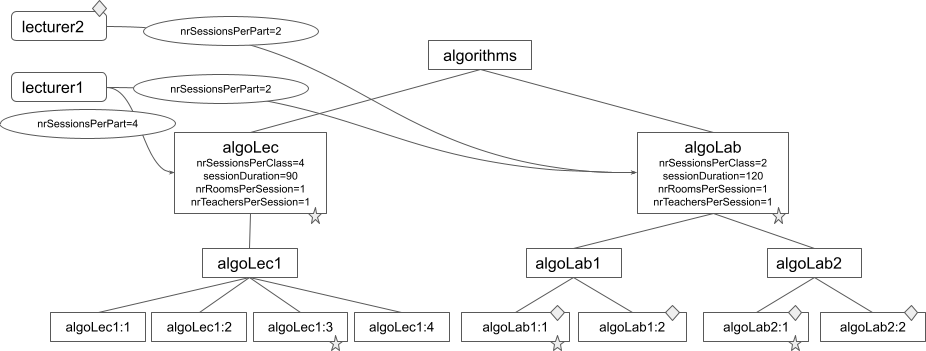
\includegraphics[scale=0.35]{img/utp_rule_1.png}


\newcounter{save_equation}
\setcounter{save_equation}{\value{equation}}
\setcounter{equation}{0}

\renewcommand{\theequation}{R\arabic{equation}}

{\footnotesize{
\begin{flalign}
&\texttt{{\FORBIDDENPERIOD}((<(\TEACHER,{lecturer2},\_)>,9120,9240)}
&\label{rule-example-1}
\\
&\texttt{{\SEQUENCED}(<(\CLASS,\_,\myset{3}),(\PART,{algoLec},\_)>,
<(\CLASS,\_,\myset{1}),(\PART,{algoLab},\_)>)}
&\label{rule-example-2}
\end{flalign}
}}


\setcounter{equation}{0}
\renewcommand{\theequation}{C\arabic{equation}}

%
{
\footnotesize
\begin{flalign}
\nonumber &\texttt{{\FORBIDDENPERIOD}((lecturer2,\{algoLab1:1,algoLab1:2,algoLab2:1,algoLab2:2\}),}\\
 & \texttt{9120,9240)}
&\label{constraint-example-1}
\\
&\texttt{{\SEQUENCED}((algoLec1,\{algoLec1:3\}), (algoLab1,\{algoLab1:1\}))}
&\label{constraint-example-2}
\\
&\texttt{{\SEQUENCED}((algoLec1,\{algoLec1:3\}), (algoLab2,\{algoLab2:1\})}
&\label{constraint-example-3}
\end{flalign}
}
%

\caption{Rules flattening and corresponding constraints on a toy example.}
\label{fig:utp-rule-1}

\setcounter{equation}{\value{save_equation}}
\end{figure}


Figure~\ref{fig:utp-rule-1} illustrates the rules flattening process on a toy example.
Course \texttt{algorithms} is split into a lecture part \texttt{algoLec} and a lab part \texttt{algoLab}.
The lecture part has a single class of 4 sessions taught by \texttt{lecturer1} and the lab part has 2 classes of 2 sessions each taught by \texttt{lecturer1} or \texttt{lecturer2}.
%Figure~\ref{fig:utp-rule-1} illustrates the flattening of the following rules: 
%on a simple model consisting of 2 teachers and & course subdivided into 2 parts, 3 classes and 8 sessions. The first rule forbids a time period for 
Rule~\ref{rule-example-1} %below
requires that \texttt{lecturer2} has no session between slots $9120$ and $9240$, corresponding for instance to 8am and 10am on Tuesday of week 2. % assuming a granularity of 1 minute per time slot. 
%In this rule, $9120$ (resp. $9240$) is the value\footnote{Each possible session schedule is mapped to a single value. All possible values make up the domain of a session.} that corresponds to 8am on Tuesday (resp. 10am on Tuesday) of week 2. 
The selector includes no mask and no filter hence matches with all possible sessions of \texttt{lecturer2} 
as indicated with diamonds on Figure~\ref{fig:utp-rule-1}. 
The resulting domain of e-maps is the singleton $\myset{(lecturer2,\map{\TEACHER}{\SESSION}{lecturer2})}$
and the rule is flattened into a single \texttt{\FORBIDDENPERIOD} constraint (\ref{constraint-example-1}). %$\myset{\map{\TEACHER}{\SESSION}{teacher2}}$.
Rule~\ref{rule-example-2}
%requires that the first practical session in Algorithmic \todo[inline]{Marc : pourquoi algo ?} start after the third lecture.
requires that the first sessions of the labs start after the third lecture.
The two selectors include a filter. The first selector matches with all class sessions of rank 3 in part \texttt{algoLec}, 
and the second matches with all class sessions of rank 1 in part \texttt{algoLab} as indicated with stars on the figure.
The rule is flattened into 2 \texttt{\SEQUENCED} constraints (\ref{constraint-example-2} and \ref{constraint-example-3}) corresponding to the cross product of the e-map domains 
%$\myset{(algoLec1,\map{\RANK}{\SESSION}{3}\cap\map{\PART}{\SESSION}{algoLec})}$
%and $\myset{(algoPra1,\map{\RANK}{\SESSION}{1}\cap\map{\PART}{\SESSION}{algoPra}),(algoPra2,\map{\RANK}{\SESSION}{1}\cap\map{\PART}{\SESSION}{algoPra})}$.
$\myset{(algoLec1,\myset{s\in\SESSION\ |\ \sessionrank{s}=3}\cap\map{\PART}{\SESSION}{algoLec})}$
and $\myset{(algoLab1,\myset{s\in\SESSION\ |\ \sessionrank{s}=1}\cap\map{\PART}{\SESSION}{algoLab}),(algoLab2,\myset{s\in\SESSION\ |\ \sessionrank{s}=1}\cap\map{\PART}{\SESSION}{algoLab})}$.
%------------------------------------------------------------
%------------------------------------------------------------
\subsection{Solution}
\label{sec:solution}
%From introduction
%{\UTP} instances may therefore be used to model subproblems and solution seeds when the whole problem is solved in successive stages (e.g., sequential workflows chaining student sectioning, course scheduling and resource allocation). 
%Since no assumption is made on the computing task, {\UTP} instances may also be used to repair timetables, complete partial timetables or generate full solutions. 

The solution component includes assignment decisions
relating to the choice of slots and resources for sessions,
the placement of students in groups and
the assignment of groups to classes.
The solution hence represented may be partial, even empty,
and does not have to be consistent with the constraints built in the entity model or entailed by the rules.
The support for partial solutions allows to tackle subproblems using separate {\UTP} instances and solution seeds.
For instance, a scheduling instance may be defined on the basis of partial and consistent solutions pre-generated for the student sectioning and resource allocation subproblems.
Likewise, the support for inconsistent solutions is paramount to repair solutions that have become inconsistent due to unforeseen changes.

%As mentioned before, 
Student groups are considered a by-product of student sectioning.
For this reason, groups may only be listed in the solution component, not in the entity model, and defined both by the students they include and the classes they are assigned to. 
This sectioning process is subject to different constraints. 
First, students are partitionned into groups and students are inextricably bound to their group.
Second, a group may only include students with identical course registrations.
Third, group-to-class assignments must comply with any subgroup inclusion constraint stated in the entity model.

%Let ${\SLOT}$ denote the range of slots defining the schedule horizon, $\maptype{\PART}{\SLOT}$ denotes the set of allowed slots defined for each course part in the entity model. 
%$\maptype{\SESSION}{\SLOT}$ shall denote the set of slots assigned to each session in a solution component.
%Let ${\GROUP}$ denote the set of groups defined in a solution, $\maptype{\GROUP}{\STUDENT}$ and $\maptype{\CLASS}{\GROUP}$ shall denote respectively the students making up each group and the groups making up each class.



% %The schema thus allows to cast university timetabling problems either as cumulative or disjunctive scheduling problems that subsume student sectioning or not.


% \paragraph{Paragraph headings} Use paragraph headings as needed.
% \begin{equation}
% a^2+b^2=c^2
% \end{equation}

% For one-column wide figures use
%\begin{figure}
% Use the relevant command to insert your figure file.
% For example, with the graphicx package use
%  \includegraphics{example.eps}
% figure caption is below the figure
%\caption{Please write your figure caption here}
%\label{fig:1}       % Give a unique label
%\end{figure}
%
% For two-column wide figures use
%\begin{figure*}
% Use the relevant command to insert your figure file.
% For example, with the graphicx package use
%  \includegraphics[width=0.75\textwidth]{example.eps}
% figure caption is below the figure
%\caption{Please write your figure caption here}
%\label{fig:2}       % Give a unique label
%\end{figure*}
%
% For tables use
%\begin{table}
% table caption is above the table
%\caption{Please write your table caption here}
%\label{tab:1}       % Give a unique label
% For LaTeX tables use
%\begin{tabular}{lll}
%\hline\noalign{\smallskip}
%first & second & third  \\
%\noalign{\smallskip}\hline\noalign{\smallskip}
%number & number & number \\
%number & number & number \\
%\noalign{\smallskip}\hline
%\end{tabular}
%\end{table}




%------------------------------------------------------------
%------------------------------------------------------------
\subsection{Related work}
\label{sec:related-work}

%Examination timetabling {1999schaerfAIR}: marginal differences with CTP => mandatory attendance for students, different workload constraints for students, can have more than one exam in a room (cumulative room), TAP {2022caselliESWA}: post-allocation of "tutors" to "workshops". BACP {2001castroARXIV,2011chiarandiniJH}: close to maquettage Student sectioning: {2010mullerAOR} => initial vs batch vs online. {2019schindlAOR} CB-CTTP {2010mccollumINFORMS,2012bettinelliAOR,2015bettinelliTOP}: week schedule  with time periods (no session duration), no modeling of student enrolments, hard: same-curriculum/teacher (disjunctive teacher/students), room occupancy, no-overlap(lectures of a course), teacher unavailabilities, soft: room capacity, room stability, ... PE-CTTP {2007lewisITC,2010mccollumINFORMS}: week schedule (45 slots) with time periods (no session duration), student sectioning factored in, each course is a single event (no series of class sessions), students and rooms disjunctive,  New/subsuming models - ITC-2019 {2018mullerPATAT}: - UCTP (survey {2021chenIEEEA}) - {2022zaulirMJFAS,2014aizamNACO} => essentially "new" workload/pattern constraints but probably encodable in ITC. General survey: {2019oudeAOR}:


We highlight here the main differences between the {\UTP} language and the {\ITC} language ({\ITC} for short).

%the two approaches use the same temporal representation but {\ITC} leaves the possibility to configure the granularity of daily slots in each instance (${\DAILYSLOT\in\myset{1\ldots 1440}}$)  while it is set to the minute in {\UTP}. Nevertheless, any granularity may be used in {\UTP} by filtering the series of allowed slots in course parts and by re-scaling session duration and travel time data.
A first difference between the two frameworks lies in the representation of the possible times a class can meet.
In {\UTP}, a class is defined by a single sequence of sessions of equal duration and the problem is to schedule each session.
In {\ITC}, a class is given alternative fixed session schedules ({\texttt{times}} elements in the {\XML} schema) and the problem is to choose one of the schedules for the class.
A schedule is the repetition over a set of weeks of one or more sessions that have the same duration and start on specific days of the week at the same predefined time (daily slot).
The two representations are not reducible to one another.
For instance, alternative schedules using different session durations cannot be modeled in {\UTP}.
Conversely, class schedules where sessions do not necessarily start on the same daily slot cannot be modeled in {\ITC}.
Nevertheless, basic class schedules may be represented in either approach by stating {\ITC} constraints or {\UTP} rules on classes.
For instance, a class meeting every week on the same day and the same daily slot, both being subject to time restrictions, may be modeled using \texttt{\SAMEDAILYSLOT}, \texttt{\WEEKLY} and \texttt{\FORBIDDENPERIOD} constraints.
The implementation of a more comprehensive reduction method %for alternative schedules 
%(based, for instance, on a dedicated {\UTP} predicate) 
will be the subject of future work.

%Another difference lies in the representation of resources and the constraints governing their distribution and allocation.
%On the one hand, 
Second, 
{\ITC} represents alternative course configurations
by introducing an intermediate layer in the course hierarchy 
that sits between courses and parts.
The configurations of a course typically differ in their number of (sub)parts
and are mutually exclusive from a student sectioning standpoint, that is, 
a registered student must be assigned a single configuration and attend all of its parts.
This feature is not currently supported in {\UTP}.
As for resources, {\UTP} explicitly represents lecturers on par with rooms %and allows to specify their workload in each course part %(i.e., the number of sessions to teach)
whereas {\ITC} only models rooms.
{\UTP} also provides the flexibility to allocate different resources within a class 
(and specify lecturer workload in particular) %(i.e., the number of sessions to teach)
whereas the same room must be allocated in {\ITC}.
Additionally, {\UTP} supports multi-resource sessions whereas {\ITC} is restricted to single-room sessions.

Lastly, the two constraint languages present important differences.
While {\ITC} constraint predicates apply to classes,
{\UTP} predicates apply to any set(s) of sessions
and may be used in particular on individual sessions, hence granting finer-grained control.
Besides, {\UTP} rules and the selector language allows to constrain any class of resources or course elements in a concise way.

Lastly, the {\ITC} schema addresses the timetabling problem as a combinatorial optimization problem.
It includes a cost function weighting 4 criteria which respectively penalize the choice of sessions and rooms for the classes, the violations of constraints and the overlapping of sessions per student.
In its current version, the {\UTP} language addresses the problem as a hard constraint satisfaction problem.
The integration of soft constraints and the possibility of aggregating penalties or preferences, either in solution generation or repair contexts, is under investigation.

%Student groups 
% near-identical course structure: no course configuration element
% no time elements in UTP classes. Alternative class times are fixed in ITC
% OK time elements in extension -> unusitable for loosely constrained class programs
% OK impossible to express k weekly slots with different starting slots. In UTP: use sameWeeklySlot with masks.
% OK impossible to enforce different constraints bettwen first period of a course (amorcage) and the rest => ok for us with masks
% KO: times with different #sessions and session length. 
% => solution per session (vs per class) : slot + romms + teachers


%Sectioning:: as itc (parent class)
%Ressources
%- rooms: travel in ITC => using constraint travel in UTP.
%- new: teachers.
%- students: no change.
%- OK groups. Admin and computational needs.
%- Domain constraints
%- by default, all resources are cumultative (explain). Avec contrainte (disjunctive):: no overlap on romms/etc. 
%- allowed slot (applies to all sessions of a part's classes) : ITC via time elements. Adequate for "grid systems". 
%- allowed rooms and allowed teachers (worklaod per part = prescribed number of sessions)
%- single or multi-room/teacher session in UTP.
%- possibly different resources between sessions of a class (unless addiiotnal rules:: sameRoom, sameTeacher, ...)
%Rules language
%- ITC: class-level constraints vs session-level constraints on UTP
%- Labelling: simplifies constraint expression to look up entities
%Solution
%seul ajout: group-to-class and student-to-group
%Résolution: UTP == SAT vs Opt/gestion prefs => pas de priorites, pondérations, etc
%

